\section{Location Access Controller}
\label{tutorial_10}

\tick{\textbf{Goals:} In this section, we will take a closer look at a few more complex proofs. For this, we will use the model of a Location Access Controller. The goal is to develop the proofs for deadlock freeness of the initial model and of the first refinement.}

%\info {First of all you need to download the following \file{Doors.zip}{Location Access Controller problem}.}

Through the model used in this section, we study a complete system and remind the proof rules of formal development. The system's task is to control the access of certain people to different locations of a site. The system is thus based on the authorization that a person has (or not has) access to a particular location.

Before the start to describe the initial model, import the archive file \file{Doors.zip}{Doors.zip} containing the model. For this select  \textsf{File $\rangle$ Import $\rangle$ General $\rangle$ Existing Project into Workspace}. Then, select the according archive file and click on \textsf{Finish}. Rodin takes a few seconds to extract and load all the files.

\subsection{Initial Model}

%Besides we introduce:

%\begin{itemize}
%	\item The two carrier sets of persons, P, and locations, L
%	\item The constant authorization, \textbf{aut}, representing a relation between P and L, actually where people are allowed to go %(Axiom 1).
%	\item The variable, \textbf{sit}, which denote where a person is, \textbf{sit} is a function from P to L.
%\end{itemize} 
 
%Moreover, we introduce a special constant “location”, named \textbf{outside}. Everyone is authorized to be in outside (Axiom 3) and a %person cannot be in two locations at a time. However every person, which is in a certain location, is authorized to be there.

%Initially, everyone is outside as indicated in event \textsf{INITIALISATION}.
%The other event \textsf{PASS} of that model has to aim to change the location of a person.
%We call the proof of deadlock freeness through this tutorial the proof justifying that someone can always change location.

Let us look at the initial model, consisting of \texttt{doors\_ctx1} and \texttt{doors\_0}. There are two carrier sets in the model context, one for people (\textsf{P}) and one for locations (\textsf{L}). Then, there is a location called outside (\textsf{outside}) where everyone is allowed to go and a relation (\textsf{aut}) which reflects where people are allowed to go. Everyone is allowed to go outside. The model machine has one event (\textsf{pass}), which changes the location of a person and one variable (\textsf{sit}), which denotes where a person is located. 

\subsection{Deadlock Freeness}

Looking through the initial model, you will see that everything already has been proved. This is true, however, Rodin does not do any deadlock freeness (\ref{deadlock_freeness}) proof yet, so we will have to add them by ourself. A model is considered as deadlocked if the system reaches a state with no outgoing transitions. The objective of this section is to develop the proofs for deadlock freeness (\ref{deadlock_freeness}) of the initial model and of the first refinement. 

Consider the event \textsf{pass} of the initial model:

\begin{description}
\EVENTS
	\EVT {pass}
		\begin{description}
		\AnyPrm
			\begin{description}
			\ItemX{ p }
			\ItemX{ l }
			\end{description}
		\WhereGrd
			\begin{description}
			\nItemX{ grd11 }{ p \mapsto  l \in  aut }
			\nItemX{ grd12 }{ sit(p) \neq  l }
			\end{description}
		\ThenAct
			\begin{description}
			\nItemX{ act11 }{ sit(p) :=  l }
			\end{description}
		\EndAct
		\end{description}
\END
\end{description}

Since, the initial model has only one event \textsf{pass}, the system might deadlock when both guards of the event (\textsf{grd11} and \textsf{grd12}) are together false. Thus, proof of deadlock freeness means proving, that someone can always change room. Clearly, we want to avoid this happening. We have thus to prove that the two guards are always true. For this add a new derived invariant to \texttt{doors\_0} called \textsf{DLF} (making it derived means clicking the \texttt{theorem} button) and change the predicate so that it is the conjunction (\ref{conjunction}) of the two guards:

\begin{description}
\INVARIANTS
	\begin{description}
		\nItemX{ DLF }{ \exists p, l\qdot (p \mapsto  l \in  aut \land  sit(p) \neq  l) }
	\end{description}
\end{description}

\info{Verweis auf ProB Plugin mit Deadlock Freeness Funktion}

Save the machine. We will see that the autoprover (\ref{autoprover}) fails to prove the theorem \textsf{DLF/THM}.

\warning{If you don't see the proof obligation \textsf{DLF/THM} maybe you forgot to mark the invariant as a theorem by clicking on the \texttt{theorem} button. Another reason that you don't see the proof obligation \textsf{DLF/THM} could be that you forgot to rename the invariant as ``DLF''.}

Let us analyze whether this is an inconsistency in the model. Switch to the \texttt{Proving Perspective } and double click on the proof obligation \textsf{DLF/THM}.

%\begin{center}
%	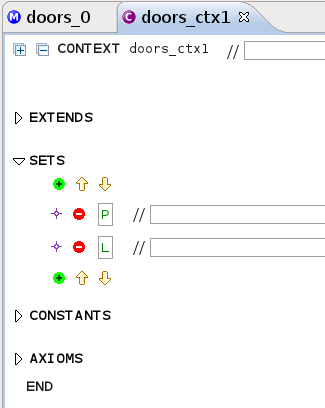
\includegraphics[]{img/tutorial/tut_10_carrier-sets.png}
%\end{center}

%\begin{center}
%	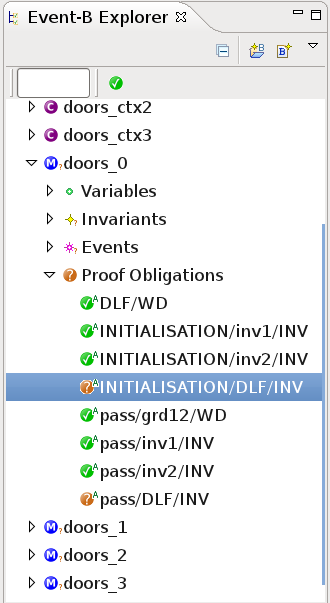
\includegraphics[]{img/tutorial/tut_10_proversfailed.png}
%\end{center}

In order to succeed with the proof, we need a tuple $p \mapsto l$ that is in \textsf{aut}, but not in \textsf{sit} ($p \mapsto l \in aut \wedge \lnot sit(p)=l$).

Searching the hypotheses, we find the Axiom 4 of \texttt{doors\_ctx1}, which states that there is a location \textsf{l}, where everyone is allowed to go. So, for every person \textsf{p} in \textsf{P}, $p \mapsto l$ and $p \mapsto outside$ is in \textbf{aut}. Since these are different, at least one of them cannot be in the function \textbf{sit}. Now, all we would need to prove is that \textsf{P} is nonempty. 

\warning{In the Proof Control view, first disable the post-tactics (there is a dedicated button in this view on the top right corner, up to the toolbar).}
\begin{center}
	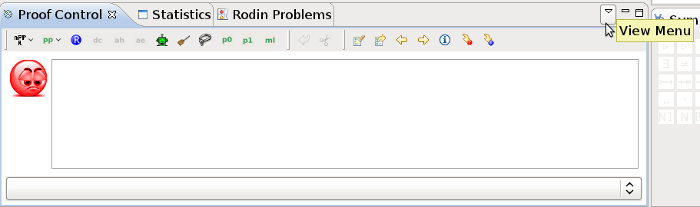
\includegraphics[]{img/tutorial/tut_10_view_menu.png}
\end{center}
We have seen that we want to prove  
\[
P \neq \emptyset
\]So we have to replace that by adding the following hypothesis in the window called \textsf{Proof Control}:
\[
\exists x.x \in P 
\]

Then click on the \textbf{ah} (Add Hypothesis) button.
\begin{center}
	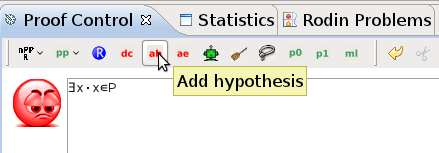
\includegraphics[]{img/tutorial/tut_10_hypothesis.png}
\end{center}


Then, click on the Auto Prover button (The button with a robot on it) until our hypothesis is selected. Actually other provers do not work here.
Once the hypothesis is in the window \textsf{Selected Hypothesis}, you can instantiate x like in the following illustration:

\begin{center}
	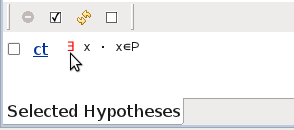
\includegraphics[]{img/tutorial/tut_10_instantiate_x.png}
\end{center}

By this action, it is automatically instantiated, and it leads to the selected hypothesis :
\[
\exists x \in P 
\]
Now we have to instantiate p in the goal with x : we enter x in the yellow box corresponding to p in the Goal view and click on the existential quantifier.

\begin{center}
	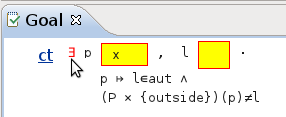
\includegraphics[]{img/tutorial/tut_10_instantiate_p.png}
\end{center}

P has been instantiated with success, however it remains to care about "l". Thus we need a case distinction.
Type sit(x) = l this into the proof control and click on Case Distinction (dc) to look at the two cases:
\[
sit(x)=l 
\]
\[
sit(x) \neq l
\]
\begin{center}
	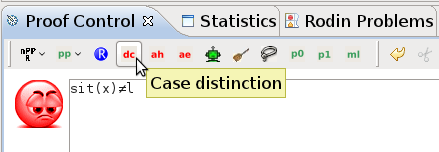
\includegraphics[]{img/tutorial/tut_10_case_distinction.png}
\end{center}

Before starting with the cases, the prover now wants you to prove that 
\[
 x \in dom(sit)
\]
This can be done with p0, as sit is a total function. In the first case x is situated in l, so it cannot be in outside. So, you can instantiate l with \textbf{outside} (type "outside" in the box corresponding to l and click on the existential quantifier). In order to prove that x is allowed to outside, you will need to select the hypothesis
\[
P \times outside \subseteq aut
\]
Now click on the lasso item in the tool bar, in order to see all of the hypotheses. Find the right hypothesis and put \textbf{outside} in the case.
\begin{center}
	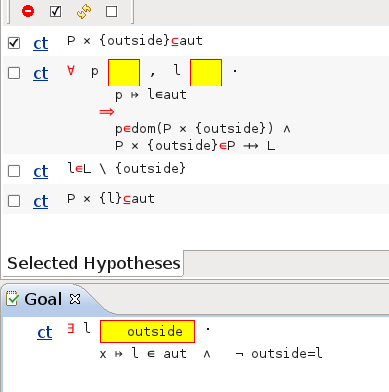
\includegraphics[]{img/tutorial/tut_10_outside.png}
\end{center}

Now click on p0, it would be proved.

\begin{center}
	
\includegraphics[]{img/tutorial/tut_10_proved.png}
\end{center}

\subsection{First Refinement}

Now we are going to detail the main complexity of our model : the deadlock freeness proof for the first refinement. 

This refinement will consist to add the new constant \textbf{com} illustrating the notion of possible direct communication between two locations.

Besides \textbf{com} is a binary relation built on the carrier set L. A location does not “communicate” with itself as stated in the Axiom 1 of the doors\_ctx2.
\[
com \in L\leftrightarrow L
\]
Concerning the events, \textsf{INITIALISATION} does not change, whereas the event \textsf{PASS} is refined as a consequence. Indeed we estimate that a person can move to another location l if there is the authorization to be in l (already defined in the abstraction) and also location l communicates with the location where p is at this precise moment (represented by sit(p)).

Consequently, the guard of this new event version is better than the precedent, since we have :

\[
( sit(p) \mapsto l \in com ) \Rightarrow ( sit(p)\neq l )
\]

In fact, we are obviously faced with a difficulty here; it is not possible to prove that the refined event \textsf{PASS} does not happen less often than its more abstract homologue. To demonstrate this, we would have to prove that the guard of the abstract event implies that of the concrete event.

The issue is that this condition cannot be verified in general. Moreover the failure to prove the above condition indicates that there are possibilities that certain people could stay permanently blocked in locations. Besides the geometry of communication between locations clearly introduces an additional constraint limiting the way people can move.

As a consequence our study has revealed a problem in our method that was obviously ignored in the document requirements.
So we must find a sufficient solution.

At the beginning of this section we need to come back to the \textsf{Event-B view}.
First of all open doors\_1 machine and add the derived invariant (theorem) called \textbf{DLF} stating :

\[
\exists q,m.(q \mapsto m \in aut \land sit(q) \mapsto m \in com )
\]
That is equivalent to say that the location sit(p) is in communication with at least one other location l, in which p is authorized to go:
the person p can therefore go out of the the location sit(p), via l, ans does not remain blocked in a location.

\begin{center}
	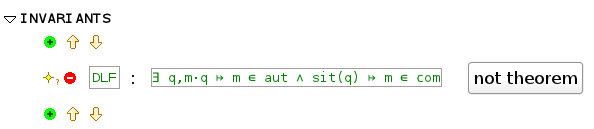
\includegraphics[]{img/tutorial/tut_10_invariants2.png}
\end{center}

Then we save the file. After switching to the proving view (the post-tactics should still be disabled), we can notice that once again, the prover fails to prove deadlock freeness automatically. 
Actually all we want is that "any person authorized to be in a location must also be authorized to go in another location which communicates with the first one".

This can be illustrated as follow:
\begin{center}
	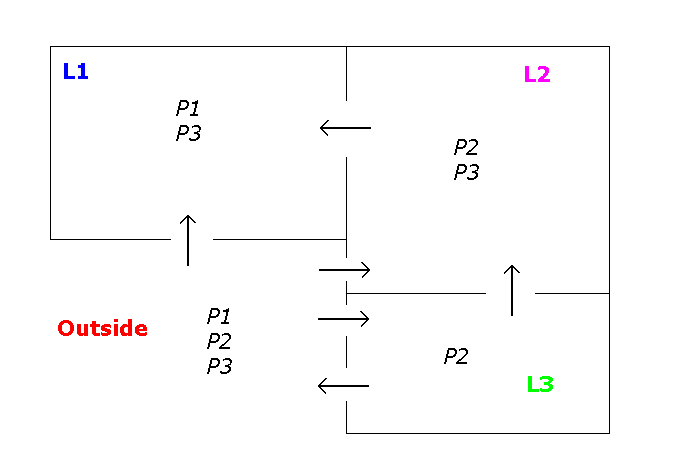
\includegraphics[]{img/tutorial/tut_10_graph.png}
\end{center}

At the beginning of the proof, there are no selected hypotheses at all. So we need to select several hypotheses. In order to complete the proof we need the old deadlock freeness invariant, and the Axiom 7 of doors\_ctx2, which will be useful too.


\[
\texttt{Axiom 7 \space \space \space \space}\exists l.l \in L \backslash \{outside\} \wedge outside \mapsto l \in com \wedge P \times \{l\} \subseteq aut
\]


But since \textbf{sit} and \textbf{aut} are inside the invariant, to begin with we also need to prove:
\[
sit \subseteq aut
\]

\[
sit \in P \mapsto L
\]
Once again, the existential quantifiers are rewritten by the auto-provers in the hypotheses. Now we will consider precisely the proof. There is an easy case if sit(p) = outside. Type this into the proof control and add this case as previously with a case distinction (dc) in order to solve it. For q, we have to select the choice p. However for m, you will use the existential quantifier of Axiom 7 to instantiate m with l as l0. 
Axiom 7 proves that we have no deadlock for people who are outside.

For the other case, we will need the notion of \textbf{exit}. This function \textbf{exit} is connecting locations to locations and defined at every location except \textbf{outside}. 
We can look at the axioms of doors\_ctx2. 
\begin{center}
	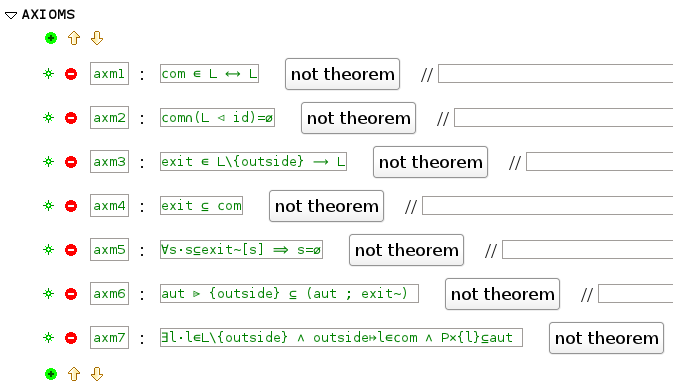
\includegraphics[]{img/tutorial/tut_10_axioms.png}
\end{center}

It states that :

\begin{itemize}
	\item (Axiom 3) Every room except the outside has exactly one exit. 
	\item (Axiom 4) An exit must be a room that communicates with the current one
	\item (Axiom 5) A chain of exits leads to the outside without any cycles or infinite paths
	\item (Axiom 6) Everyone allowed in a room is allowed to go through its exit. 
\end{itemize}  

In our proof, we still need to show that anyone who is not outside can walk through a door. For this, Axiom 5 is useless, so we add all hypotheses containing exit except for Axiom 5. Now we have to instantiate q and m correctly and to conclude that the proof should not be too hard. Once again, for q, the choice p is obvious. But it is not quite as easy for m. Expressed in language, m must be the room behind the exit door of the room that p is currently in. 

\info{Try translating this into set theory. But do not worry if you get it wrong. You can still go back in the proof by right-clicking at the desired point in the proof tree and choosing prune in order to retry.}
\begin{center}
	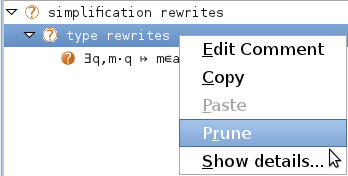
\includegraphics[]{img/tutorial/tut_10_prune.png}
\end{center}

